%%%%%%%%%%%%%%%%%%%%%%%%%%%%%%%%%%%%%%%%%
% University Assignment Title Page 
% LaTeX Template
% Version 1.0 (27/12/12)
%
% This template has been downloaded from:
% http://www.LaTeXTemplates.com
%
% Original author:
% WikiBooks (http://en.wikibooks.org/wiki/LaTeX/Title_Creation)
%
% License:
% CC BY-NC-SA 3.0 (http://creativecommons.org/licenses/by-nc-sa/3.0/)
% 
% Instructions for using this template:
% This title page is capable of being compiled as is. This is not useful for 
% including it in another document. To do this, you have two options: 
%
% 1) Copy/paste everything between \begin{document} and \end{document} 
% starting at \begin{titlepage} and paste this into another LaTeX file where you 
% want your title page.
% OR
% 2) Remove everything outside the \begin{titlepage} and \end{titlepage} and 
% move this file to the same directory as the LaTeX file you wish to add it to. 
% Then add \input{./title_page_1.tex} to your LaTeX file where you want your
% title page.
%
%%%%%%%%%%%%%%%%%%%%%%%%%%%%%%%%%%%%%%%%%
%\title{Title page with logo}
%----------------------------------------------------------------------------------------
%	PACKAGES AND OTHER DOCUMENT CONFIGURATIONS
%----------------------------------------------------------------------------------------

\documentclass[12pt]{article}
\usepackage{wrapfig}
\usepackage[english]{babel}
\usepackage[utf8]{inputenc}
\usepackage{amsmath}
\usepackage{graphicx}
\usepackage[colorinlistoftodos]{todonotes}

\begin{document}

\begin{titlepage}

\newcommand{\HRule}{\rule{\linewidth}{0.5mm}} % Defines a new command for the horizontal lines, change thickness here

\center % Center everything on the page
 
%----------------------------------------------------------------------------------------
%	HEADING SECTIONS
%----------------------------------------------------------------------------------------

\textsc{\LARGE Universidad de Sonora }\\[0.3cm] % Name of your university/college
\textsc{\Large Departamento de Ciencias Naturales y Exactas  }\\[0.3cm]
\textsc{\Large Licenciatura en Física }\\[0.3cm]
\textsc{\Large Física computacional I}\\[0.3cm] % Major heading such as course name
 % Minor heading such as course title

%----------------------------------------------------------------------------------------
%	TITLE SECTION
%----------------------------------------------------------------------------------------

\HRule \\[0.1cm]
{ \huge \bfseries Actividad 2\\  Introducción a Python, Jupyter y Panda}\\[0.01cm] % Title of your document
\HRule \\[1.5cm]

 
%----------------------------------------------------------------------------------------
%	AUTHOR SECTION
%----------------------------------------------------------------------------------------

\begin{minipage}{0.4\textwidth}
\begin{flushleft} \large
\emph{Alumno:}\\
Gómez García \\Manuel Ignacio\\ %Grupo 1 % Your name
\end{flushleft}
\end{minipage}
~
\begin{minipage}{0.4\textwidth}
\begin{flushright} \large
\emph{Profesor:} \\
Lizarraga Celaya\\Carlos\\%Dept. of CSE % Supervisor's Name
\end{flushright}
\end{minipage}\\[1cm]

% If you don't want a supervisor, uncomment the two lines below and remove the section above
%\Large \emph{Author:}\\
%John \textsc{Smith}\\[3cm] % Your name

%----------------------------------------------------------------------------------------
%	DATE SECTION
%----------------------------------------------------------------------------------------

{\large \date[21 de febrero, 2018 \\Hermosillo, Sonora}\\[1cm] % Date, change the \today to a set date if you want to be precise

%----------------------------------------------------------------------------------------
%	LOGO SECTION
%----------------------------------------------------------------------------------------


\includegraphics[height=5.5cm]{Logo}\\[0.5cm] % Include a department/university logo - this will require the graphicx package
 
%----------------------------------------------------------------------------------------

\vfill % Fill the rest of the page with whitespace

\end{titlepage}


%\begin{abstract}
%Your abstract.
%\end{abstract}
\begin{titlepage}
\title {Jupyter not\ebook}
\end{titlepage}

\section{Introducción}

En la presente práctica de Python, hicimos uso de Jupyter notebook en conjunto con las bibliotecas de Panda, Numpy, Matplotlib para realizar un análisis de datos correspondiente con los proporcionados por las "Estaciones Automatizadas del Servicio Meteorológico Nacional".
\\
\\ Además del análisis de datos, otro objetivo de la práctica es conocer Jupyter Notebook, el cual es una aplicación Open-Source en línea, usada principalmente para crear y editar archivos con la finalidad de analizar datos, simulaciones numéricas, transformaciones, machine learning y otros más. 

\section{Realización de la Actividad 2}
Para la actividad 2 seguimos los pasos mostrados en el repositorio de GitHub que se indicaba en el portal de computacional. Al seguir los pasos mostrados en el archivo el objetivo es conocer y familiarizarnos con los comandos usados en la práctica, además al final se nos pide que generemos tres distintas gráficas para analizarlas, posteriormente describimos dichos gráficos.
\\
\\ Las gráficas generadas son las siguientes:
\begin{itemize}
\item Rapidez de los vientos y de las ráfagas como funciones del tiempo.
\begin{figure}[h!]
\begin{center}
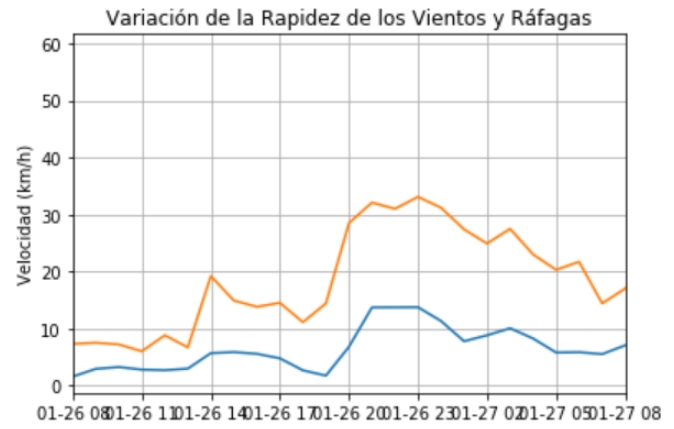
\includegraphics[height=6cm]{Vel}%\\[1cm]
\end{center}
\end{figure}

\item Dirección de los vientos como función del tiempo.
\begin{figure}[h!]
\begin{center}
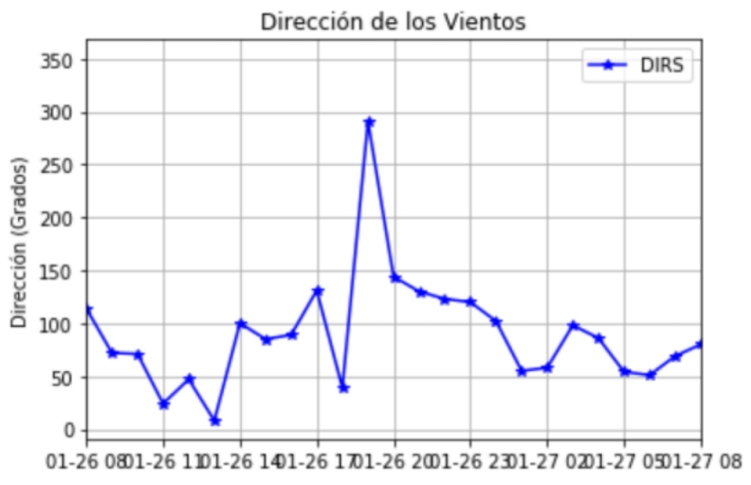
\includegraphics[height=6cm]{Dir}
\end{center}
\end{figure}

\item Radiación solar como función del tiempo.
\begin{figure}[h!]
\begin{center}
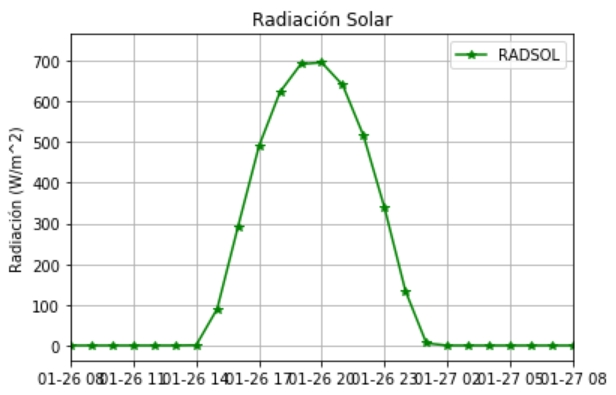
\includegraphics[height=6cm]{Rad}
\end{center}
\end{figure}

\end{itemize}

\subsection{Preguntas de la Actividad}
\begin{enumerate}
\item ¿Cuáles son las horas del día con más viento?
\medskip
\\ En base a la gráfica mostrada de las velocidades en función del tiempo, podemos determinar que entre las 12:00 y 15:00 es cuando las velocidades alcanzan sus máximos.

\item Comentar sobre los vientos dominantes en el sitio de estudio.
\medskip
\\ Al analizar durante 24 horas el municipio de Tecate, Baja California Norte vemos como la velocidad promedio de los vientos es de 7 km/h mientras que la de las ráfagas es de 19 km/h.

\item En base al comportamiento de la radiación solar. ¿Qué puedes comentar?
\medskip
\\ Como era de esperarse, las mayor cantidad de radiación se da entre las 11:00 y 12:00, por otro lado, la radiación es prácticamente nula de 00:00 - 6:00 y de 17:00 - 24:00; también podríamos decir que la gráfica se asemeja a una gaussiana.

\item ¿Cuál es el lapso de temperatura diaria? (Diferencia entre la temperatura máxima y la mínima).
\medskip
\\ La comparativa de los datos muestra que la diferencia entre la temperatura máxima y mínima registrada a lo largo del día fue de 13 $^{\circ}$C, siendo la máxima de 18 $^{\circ}$C y la mínima de 5 $^{\circ}$C.

\item ¿Puedes comentar sobre la relación entre la temperatura y la humedad relativa?
\medskip
\\ Se puede ver en la tabla (o en una gráfica) que conforme aumenta la temperatura disminuye la humedad relativa pero dicho proporción no es tan notoria al paso del día.

\end{enumerate}

\section{Características de Jupyter Notebook}
Jupyter Notebook es una aplicación muy usada por diversos aspectos que lo favorecen a comparación de otros softwares existentes. Entre las características que lo hacen destacar tenemos... 
\begin{itemize}
\item El hecho de que es un software de código abierto es de gran utilidad para todo mundo.

\item Es muy fácil manejar el programa en sí.

\item Los archivos que creamos desde la aplicación son sencillos de compartir, inclusive con aplicaciones de terceros.

\item Es posible el realizar un trabajo colectivo remotamente entre los participantes.
\item No existe necesidad alguna de instalar el software para hacer uso de éste, basta simplemente con tener acceso a internet.

\item Jupyter es compatible, no sólo con Python, sino con cuarenta lenguajes más, entre ellos R, Julia y Scala.

\item Podemos trabajar en tiempo real conforme avanzamos en nuestro documento, con la visualización de imágenes, videos, \LaTeX y JavaScript.

\end{itemize}

\section{Limitaciones de Jupyter Notebook}
Una limitación que presenta Jupyter es que no es posible cambiar el nombre del notebook que hemos creado debido a cierto protocolos con los cuales es incompatible la aplicación.

\section{Apéndice}
\begin{enumerate}
\item ¿Cuál es tu primera impresión de Jupyter Notebook? 
\medskip
\\ Me pareció asombroso el ver cómo ingrese a la aplicación, también me parece un excelente programa por el hecho de que es posible crear desde la misma todos los archivos que necesitamos y utilizar diversos lenguajes de programación.
\\Otro aspecto que me asombró fue el poder trabajar sin necesidad de instalar el programa, usando una conexión a internet.

\item ¿Se te dificultó leer código en Python?
\medskip
\\ No me parece que sea díficil comprender los comandos de Python, son sencillos de comprender y uno puede familiarizarse con ellos rápidamente, simplemente es cuestión de prácticar.

\item ¿En base a tu experiencia de programación en FORTRAN, que te parece el entorno de trabajo en Python?
\medskip
\\ Se siente distinto dado que en FORTRAN al ser un lenguaje de compilado es necesario crear todo nuestro código entero para posteriormente probar que el código tenga una sintaxis correcta y que de igual forma su estructura, mientras que por otro lado Python es del tipo interpretativo, lo que significa que es posible compilar y probar cada renglón o segmento de código, según como queramos.
\\ Por otro lado, tenemos la opción de agregar bibliotecas (conjunto de funciones) al archivo a trabajar, las cuales desconocía en FORTRAN, para así tener opciones específicas con otros comandos.

\item A diferencia de FORTRAN, ahora se producen las gráficas utilizando la biblioteca Matplotlib. ¿Cómo fue tu experiencia?
\medskip
\\ El hecho de poder generar las gráficas ahí mismo, la forma de hacerlo, todo eso me parece bastante útil al desear analizar los datos con los que contamos para apreciarlos visualmente.

\item En general, ¿qué te pareció el entorno de trabajo en Python?
\medskip
\\ Python parece bastante fácil de usar, no existe gran dificultad al momento de comprender el código fuente o el crearlo y el hecho de poder compilar cada renglón nos permite ver cómo vamos en cada pedazo de archivo que estamos creando.

\item ¿Qué opinas de la actividad? ¿Estuvo compleja? ¿Mucho material nuevo? ¿Que le faltó o que le sobró? ¿Qué modificarías para mejorar?
\medskip
\\ La actividad fue interesante para comenzar a utilizar comandos para el análisis de datos y generar gráficos, siento que estuvo bastante bien en cuanto al material que mostraba y no creo necesario modificar algo al respecto de ella.

\item ¿Comentarios adicionales que desees compartir?
\medskip
\\ En lo personal, no tengo comentario alguno que hacer al respecto.

\end{enumerate}

\end{document}